\documentclass[conference]{IEEEtran}
\usepackage{graphicx}


\begin{document}

\title{Towards the Internet of Things: A Real-World Testbed}
\author{\IEEEauthorblockN{Nacer Khalil}
\IEEEauthorblockA{School of Electrical and Engineering\\
Al Akhawayn University In Ifrane\\
Email: n.khalil@aui.ma}
\and
\IEEEauthorblockN{Mohamed Riduan Abid}
\IEEEauthorblockA{School of Electrical and Engineering\\
Al Akhawayn University In Ifrane\\
Email: r.abid@aui.ma}
\and
\IEEEauthorblockN{Driss Benhaddou}
\IEEEauthorblockA{School of Engineering and Technology\\
University of Houston\\
Email: dbenhaddou@uh.edu}}
\maketitle
\begin{abstract}
The internet has seen its importance grow exponentially throughout the previous two decades. It has started as set of computers sharing static information written by human beings and accessed by other human beings. It followed mainly the publisher subscriber model. Later on, with the arrival of internet 2.0, the subscriber had now the ability to affect the content at the publisher's level and this basic idea gave rise to a whole new world of applications such as wikis, blogs, social networks and other applications. The next revolution in the internet is the introduction of machines as players within the internet. This will allow the machines to intercommunicate between them or what is known as machine-to-machine communication. More and more devices will be able to communicate and thus be part of the internet. This will give rise to a whole new dimension of possibilities as the focus of the internet will not only be human interactions but also machine interactions. As an example of autonomous machines communicating through, the components of smart grids will be part of the internet of things. Devices such as AMI, smart homes, wireless sensor networks will all be part of the internet of things. Any device within the smart grid will be uniquely identified through the network and therefore will be able to communicate. In this paper, we present a real-world testbed for integrating wireless sensors into the internet. The solution uses 6lowPAN, and addresses relevant issues at the level of the gateway. we used legacy hardware and proved communication.
\end{abstract}

\begin{IEEEkeywords}
WSN, 6lowPAN, TinyOS, IOT, cyber physical systems
\end{IEEEkeywords}

%\IEEEpeerreviewmaketitle
\section{Introduction}
The direction that is taken by the global society is a direction leading to what is known by "always connected" model. People are eager to receive the information as fast as possible and whenever available. They also want to send information as fast as possible and whenever wanted. Also, these requests and responses that are dictated by the human are not all the time directed towards humans , but can be sent also to devices and machines but that is not always possible at this time being. The future  of internet goes into this direction: being able to connect human beings as well as machine in order to provide robust and flexible communication for all. The machines on the other hand need an interface to be able to communicate on the internet. In this paper, we create a small network where a machine-to-machine communication is possible. This can be part of what is known as internet of things. The testbed created is composed of a wireless sensor network(WSN), a middleware station and a mobile client within the field of smart grids where data is collected from the motes within the WSN and sent to the middleware. The mobile client accesses this data and the mobile client can send messages directly to any mote within the WSN network in order to turn on or off any appliance. The issues that were handled are the following:
\begin{itemize}
\item The system is developed using heterogeneous networks, different data link layer technologies
\item The WSN uses IPV6 over 6lowPAN whereas other components of the system use IPV4
\end{itemize}
To solve these issues, different programs have been used to deal with these issues. 
 
\section{Literature review}

\section{Internet of things}
The internet of things is a new concept based on the idea that there will be much more users that are computers, machine than human beings. This means that machines will play an important role in the internet and they will be able to communicate autonomously without the interaction of human beings. Wireless sensor network will be part of the internet of things and therefore will be actively communicating in the internet by sending sensor data. Nowadays, the internet is mainly based on a human-to-human. In the future of internet called the internet of things, we will have in addition to human-to-human communication, human-to-machine communication and machine-to-machine communication. An example of human-to-machine communication is when the human will be able to control the wireless sensor network's sampling time. An example of machine-to-machine communication which will be discussed in this paper is the middleware being able to turn off the light because no one is in the room. The middleware by making use of the sensor data will communicate with motes to turn on or off the light bulb.
\section{6lowpan}
6loWPAN stands for  "IPv6 over Low power Wireless Personal Area Networks". It stands for the name of the working group within IETF. It is based on the idea that all the devices independently of their processing power or energy resources should be able to have the TCP/IP protocol stack and be part of the internet of things. In order to be able to build the TCP/IP protocol stack in low-power devices, there have been multiple aspects of the protocol stack that has to be optimized. As an example, the IP MTU(maximum transmission unit) is fixed at 1280 bytes whereas the Zigbee MTU is only 127 bytes. This means that not every IPV6 packet can be inserted within a Zigbee frame. Another issue is related to the addressing with the 128 bits address. in 6lowpan, the addressing via the IPV6 address is performed hierarchically to first identify is the packet is sent to a device within that network but afterwards, addressing is done by counting mainly on the 16 last bits of the IPV6 address. These were just two of a large set of issues that 6lowpan tries to solve in order to enable even the low-power devices to join the internet of things. TinyOS as being one of the most used operating system comes with its implementation of 6lowpan through a project called BLIP (Berkeley Low-power IP stack) that provides a lightweight implementation of the 6lowpan and that can be installed and used with a variety of motes as long as they support IPV6. This project makes use of BLIP to provide the TCP/IP protocol stack to the devices within the wireless sensor network.
\section{Architecture}
The project is composed of three building blocks. 
\begin{itemize}
\item Wireless sensor network (WSN)
\item Gateway server
\item Middleware
\item Mobile client
\end{itemize}
The WSN communicates using zigbee as well as with the gateway server using IPV6 technology whereas whereas the communication between the gateway server, the middleware and the mobile client is done via Wifi using IPV4 technology. The architecture enables any component within this system to communicate with any other system independently of the communication medium used (Zigbee or Wifi) or the network technology used (IPV4 or IPV6). Figure 1 is a network diagram that depicts the different components of the system as well as the routes that exist for any component to communicate with another.

\begin{figure}[htbp]
\centering
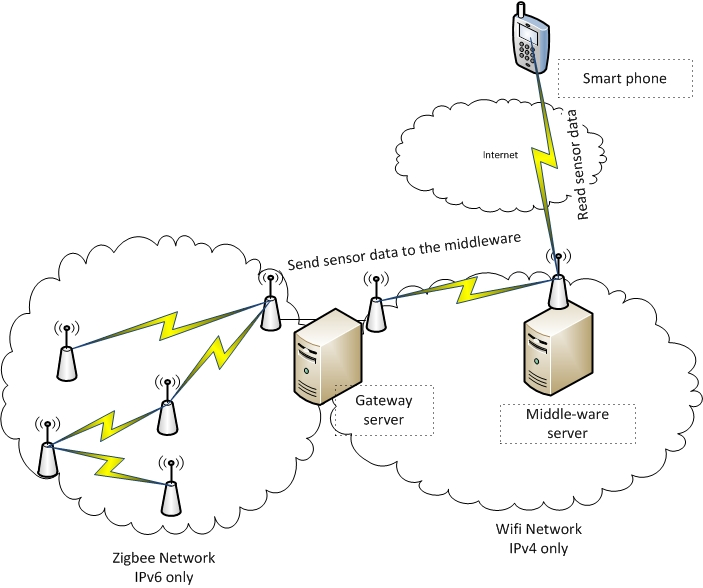
\includegraphics[scale=0.5]{images/network_diagram.jpg}
\caption{Network diagram}
\label{fig:network}
\end{figure}

\subsection{Wireless sensor network}
The wireless sensor network is based on the mesh topology. It is also designed in order to be an ad-hoc network. This means that you can place the mote any where as long as there is one link it can attain to communicate with. The routing is multi-hop and links are created dynamically between different motes of the WSN.
\section{Implementation}
To have a system that is capable of providing a two-way communication between any host and the any mote within the wireless sensor network, four building blocks had to be provided and which are the following:
\begin{itemize}
\item Mote programming
\item Mote sink packet forwarding
\item Network gateway packet transformation
\item Network gateway sensor data server
\end{itemize}

\subsection{Mote programming}
Each mote within the WSN network is equipped with a current transformer that is attached to data acquisition board through which data is read and transformed to the appropriate format and sent to the network host. In addition to this, the appliance is attached to the mote through the relay pins existing within the data acquisition board in the mote. In other words, the mote can control the electricity going to each mote and can allow it or block it. This means that one can control the appliance by using some of the functionalities provided by the mote. From the mote's perspective there are two parts that are implemented within its TinyOS program. A TCP server that is used to receive on/off requests in order to control the mote and a TCP client used to send sensor data.Once the program installed, an IPV6 address is passed to the installation routine in order to assign a static IPV6 address to the mote in which the program is cross-compiled and installed. The TCP server and TCP client work in parallel as each one's traffic is handled separately.

\subsubsection{TCP server}
The TCP server is an important component in the mote's program. Any one willing to control the appliance must connect to the TCP server and send requests. As a mote may control more than one appliance, we then identify the appliance by a unique id and send a zero to turn off or one to turn on. Requests such as "1 1" means to turn on the appliance with id 1.
\subsubsection{TCP Client}
The TCP Client is an important component in the mote's program. It serves as mean to send sensor data to the gateway reliably. Once the mote is turned on, the client connects to a TCP server that is in the gateway, then the consumption data is sensed periodically (once per second) and sent to the TCP server who deals with the sensor data.

\subsection{Mote sink packet forwarding}
The mote sink packet forwarding module is a special program installed within a mote that is equipped with a USB port that plays the role of a network interface card. The mote is attached to the gateway station and has the BLIP (Berkeley Low power IP stack Protocol) module within in. In addition it communicates with the gateway using USB protocol. In the gateway station, the network interface module is a sort of a IPV6 over USB tunnel which means that if an IPV6 packet packet is going to the sink, it is encapsulated within a USB frame and once it arrives to the mote, the IPV6 packet is extracted and forwarded to the destination mote holding that IPV6 address. The other way around is fairly similar, when a mote wants to send an IPV6 packet to the outside world, the mote creates the packet, sends it to the sink that forwards it by encapsulating it into a USB frame.

\subsection{Network gateway packet transformation}
This is a very important component in the system. The issue is the following. The WSN network supports only IPV6 while other components such as the middleware and the mobile client do not necessary have an IPV6 address, but we still want all the components to communicate independently of the IP technology to be used. To do so, we have created a network packet transformation program. This program basically converts IPV4 to IPV6 and vice versa. To do so, it assigns virtual IPV4 addresses to IPV6 address holders and and IPV6 address to IPV4 address holders. With such a program, each player in the network has both an IPV4 and an IPV6 but is aware of only the one that is assigned to him. The other "virtual" address is known only at the level of the program installed at the gateway station between the WSN and the outside world. The flow of information works as follow; when a station wants to send requests to a mote, it will send IPV4 packet holding the request to the mote but by addressing it using its virtual IPV4 address. This packet will be sniffed by this packet transformation program that will extract the TCP datagram from the ip packet, create a new IPV6 packet specifying the source address as the virtual address of the host and the destination as the address of the mote and then append the TCP datagram to the newly created packet and send it to the mote sink packet forwarding component that is seen by the gateway as a network interface card. This leads to a complicated issue that is to be handled and which is that the program should keep track of the request responses in order to forward them correctly to the destination. To solve such a problem, an algorithm has been created whose sole role is to mechanically compute the IPV6 address of the host based on its IPV4 and vice versa. This algorithm is based on function whose primary quality is the fact that it is bijective which means any IPV4 address is mapped to one and only one IPV6 function and vice versa. So whenever a request is coming, the source and destination address will be converted using this algorithm and this will make avoid the whole request response tracking part.
\section{Measurements}

\section{Conclusion}
The conclusion goes here.

\begin{thebibliography}{1}

\bibitem{IEEEhowto:kopka}
H.~Kopka and P.~W. Daly, \emph{A Guide to \LaTeX}, 3rd~ed.\hskip 1em plus
  0.5em minus 0.4em\relax Harlow, England: Addison-Wesley, 1999.

\end{thebibliography}

\end{document}


